\documentclass[a4paper, 12pt]{article}
\usepackage{graphicx}

\begin{document}
\title{Project Requirements}
\author{Felgenhauer, Maximilian\\
  \and
  Klose, Anthony\\
  \and
  Marten, Jameson}
\date{September, 24, 2012}

\maketitle

\section{Introduction}

\begin{enumerate}
\item{Purpose of the System}\\
  The purpose of this system is to facilitate writing Java code by modelling class structures in UML.

\item{Scope of the System}\\
  This system is intended for Java programmers and program designers.

\item{The success criteria of the project}\\
  To create a functioning program which can diagram UML and translate UML into Java code.
\end{enumerate}

\section{Proposed System}

\begin{enumerate}
\item{Functional Requirements}\\
  A user must be able to create and edit UML diagrams.\\
  A user must be able to read and write diagrams to a file.\\
  A user must be able to generate Java code from UML diagrams.\\
  A user must be able to make UML templates.\\

\item{Nonfunctional Requirements}
  \begin{enumerate}
  \item{Usability}
    \begin {itemize}
      \item This application should look native to the Windows or Mac, based on the operating system used.
      \item There should be a maximum of 2 steps to create any UML element. 
      \item Program will have a Single Document Interface.
    \end {itemize}

  \item{Reliability}
    \begin {itemize}
      \item The program will report any errors to the user instead of crashing, if possible.
    \end {itemize}

  \item{Performance}
    \begin{itemize}
      \item Should take the User no longer than 3 seconds to save a document.
      \item Adding GUI elements should be instantaneous. %check
    \end{itemize}
  \end{enumerate}
\end{enumerate}


%Use cases
\section{Use Case Model}


\begin{center}
  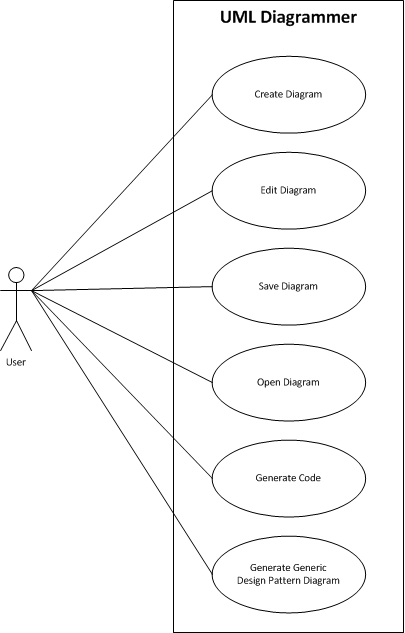
\includegraphics[height=5in,width=3in]{img/SystemOverview.png}
\end{center}

\begin {center}
  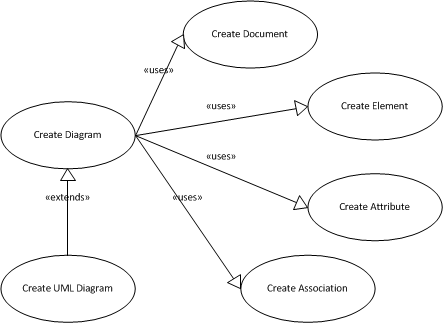
\includegraphics[height=3in, width=5in]{img/CreateDiagram.png}
\end{center}

\begin{enumerate}
\item Create UML Class Elements
  \begin {enumerate}
  \item Priority level: High
  \item Participating Actors
    \begin{itemize}
    \item User
    \item System
    \end {itemize}
  \item Flow of Events
    \begin {enumerate}
    \item User clicks somewhere on the document
    \item System creates UML Class at the point on the screen the user clicked
    \end {enumerate}
  \item Entry Conditions
    \begin {itemize}
    \item User presses Edit/Create/UML Class
    \item User presses Right Click/Create/UML Class
    \end {itemize}
  \item Exit Conditions
    \begin {itemize}
    \item UML Class is created
    \end {itemize}
  \end {enumerate}

  \begin{center}
    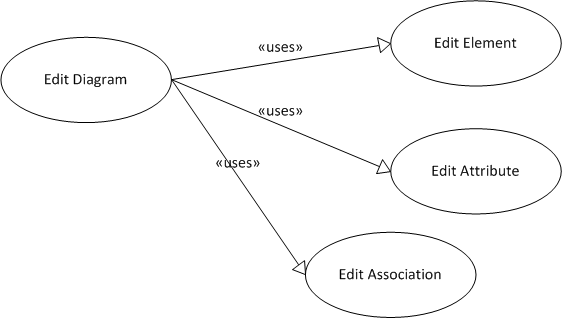
\includegraphics[height=3in, width=5in]{img/EditDiagram.png}
  \end{center}

\item Edit UML Class Elements
  \begin {enumerate}
  \item Priority Level: Medium
  \item Participating Actors
    \begin {itemize}
    \item User
    \item System
    \end {itemize}
  \item Flow of Events
    \begin {enumerate}
    \item System prompts User with a Edit Element Window
    \end {enumerate}
  \item Entry Conditions
    \begin {itemize}
    \item User right click Element/Edit/Add attribute
    \item User clicks Edit/Add/Attribute
    \end {itemize}
  \end {enumerate}

  \begin {center}
    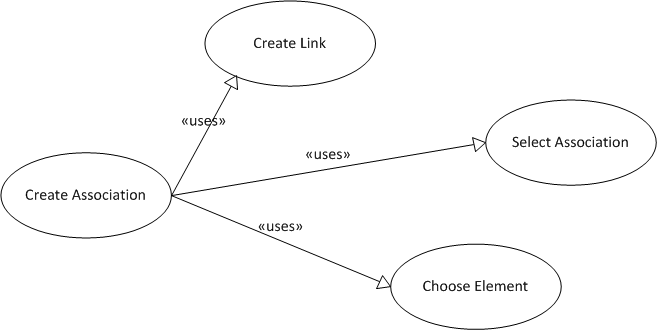
\includegraphics[height=3in, width=5in]{img/CreateAssociation.png}
  \end {center}

\item Create Association
  \begin {enumerate}
  \item Priority Level: High
  \item Participating Actors
    \begin {itemize}
    \item User
    \item System
    \end {itemize}
  \item Flow of Events
    \begin {enumerate}
    \item User will select which type of association
    \item User will select one UML element
    \item User will select a second UML element that is not the first
    \item System creates a link between the two elements
    \end {enumerate}
  \item Entry Conditions
    \begin {itemize}
    \item User Clicks Edit/Create/Association
    \item User Right clicks first element
    \end {itemize}
  \item Exit Conditions
    \begin {itemize}
    \item User cancels
    \item Link has been created
    \end {itemize}
  \end {enumerate}

  \begin {center}
    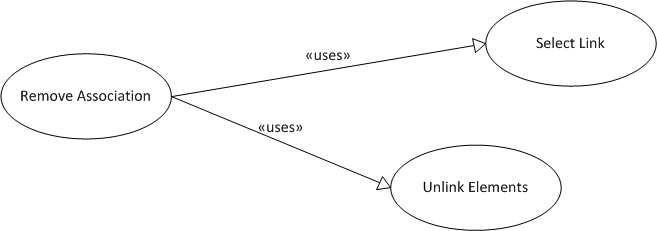
\includegraphics[width=5in, height=3in] {img/RemoveAssociation.png}
  \end {center}

\item Remove Association
  \begin {enumerate}
  \item Priority Level: High
  \item Participating Actors
    \begin {itemize}
    \item User
    \item System
    \end {itemize}
  \item Flow of Events
    \begin {enumerate}
    \item User selects an association
    \item System unlinks the elements
    \end {enumerate}
  \item Entry Conditions
    \begin {itemize}
    \item User Clicks Edit/Association
    \end {itemize}
  \item Exit Conditions
    \begin {itemize}
    \item Link has been removed
    \end {itemize}
  \end {enumerate}

  \begin{center}
    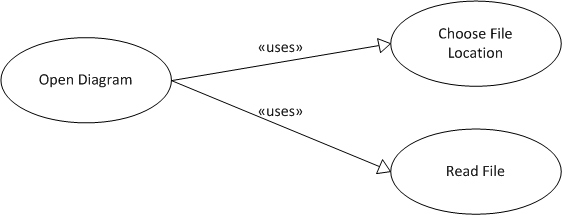
\includegraphics[height=2in, width=3in]{img/OpenDiagram.png}
  \end{center}

\item Open File
  \begin {enumerate}
  \item Priority Priority Level: Medium
  \item Participating Actors
    \begin {itemize}
    \item User
    \item System
    \end {itemize}
  \item Flow of Events
    \begin {enumerate}
    \item System prompts User for a filename that exists on the System
    \item User picks filename
    \item System opens a new document with the contents of the file
    \end {enumerate}
  \item  Entry Conditions 
    \begin {itemize}
    \item User presses File/Open
    \end {itemize}
  \item Exit Conditions
    \begin {itemize}
    \item User chooses filename
    \item User cancels
    \end {itemize}
  \end {enumerate}

  \begin {center}
    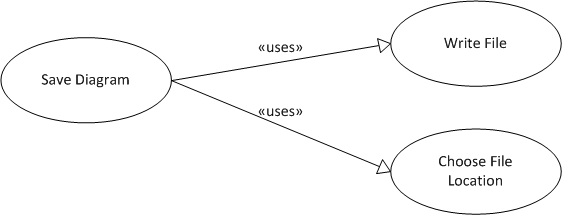
\includegraphics[height=2in,width=3in]{img/SaveDiagram.png}
  \end {center}

\item Write File
  \begin {enumerate}
  \item Priority level: Medium
  \item Participating Actors
    \begin {itemize}
    \item User
    \item System
    \end {itemize}
  \item Flow of Events
    \begin {enumerate}
    \item System prompts User for new or existing filename
    \item User enters a filename
    \item System saves document to a file on the system
    \end {enumerate}
  \item Entry Conditions
    \begin {itemize}
    \item User presses File/Save
    \item User presses File/Save as. . .
    \item User presses Save button
    \end {itemize}
  \item Exit Conditions
    \begin {itemize}
    \item User specifies a file
    \item User cancels
    \end {itemize}
  \end {enumerate}



\item Generate Java Skeletons
  \begin {enumerate}
  \item Priority level: High
  \item Participating Actors
    \begin {itemize}
    \item User
    \item System
    \end {itemize}
  \item Flow of Events
    \begin {enumerate}
    \item System creates Java files
    \end {enumerate}
  \item Entry Conditions
    \begin {itemize}
    \item User presses File/Export/Java Project
    \item User presses Right click/Export/Java Porject
    \end {itemize}
  \item Exit Conditions
    \begin {itemize}
    \item System is done writing Java files
    \end{itemize}
  \end {enumerate}

  \begin{center}
    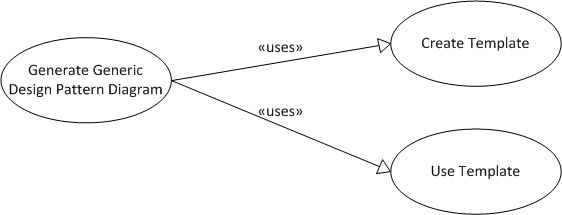
\includegraphics[height=2in,width=3in]{img/CreateGenericDesignPatternDiagram.png}
  \end{center}

\item Create UML Template
  \begin {enumerate}
  \item Priority level: Low
  \item Participating Actors
    \begin {itemize}
    \item User
    \item System
    \end {itemize}
  \item Flow of Events
    \begin {enumerate}
    \item System prompt user for name of the template
    \item system saves current document into templates file
    \end {enumerate}
  \item Entry conditions
    \begin {itemize}
    \item Document is not empty
    \item User presses File/Templates/Create
    \end {itemize}
  \item Exit Conditions
    \begin {itemize}
    \item System finishes saving file
    \end {itemize}
  \end {enumerate}

  \begin {center}
    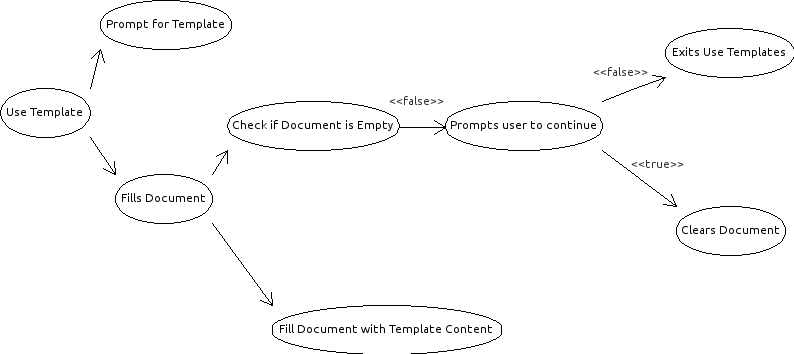
\includegraphics[width=5in, height=3in] {img/UseTemplate.png}
  \end {center}

\item Use UML Template
  \begin {enumerate}
  \item Piroity level: Low
  \item Participating Actors
    \begin {itemize}
    \item User
    \item System
    \end {itemize}
  \item Flow of Events
    \begin {enumerate}
    \item Prompt user for which template to fill the document
    \item If current document is not empty, system prompts the user if he/she wants to continue
    \item If current document is not empty, clear it
    \item Fill current document with template
    \end {enumerate}
  \item Entry Conditions
    \begin{itemize}
    \item User presses File/Templates/Open
    \end {itemize}
  \item Exit Conditions
    \begin {itemize}
    \item User decides to not continue
    \item System finishes loading template
    \end {itemize}
  \end {enumerate}
\end {enumerate}
\end{document}
